% Chapter 7

\chapter{Block Diagram}
\label{Chapter7}

As interrupts come from sources (from the same or different sources), we also tell whether the interrupt is \textbf{ Level or edge triggered}? Then gateway passes these intterupts to target in the form of ip (interrupt  pending).

\par
Target then segregates the interrupts with respect to their priority. Then finally, using valid-ready interface  interrupt is sent to RISC-V processor to service it. High priority interrupt is serviced first.

\begin{figure}[h]
  \centering
  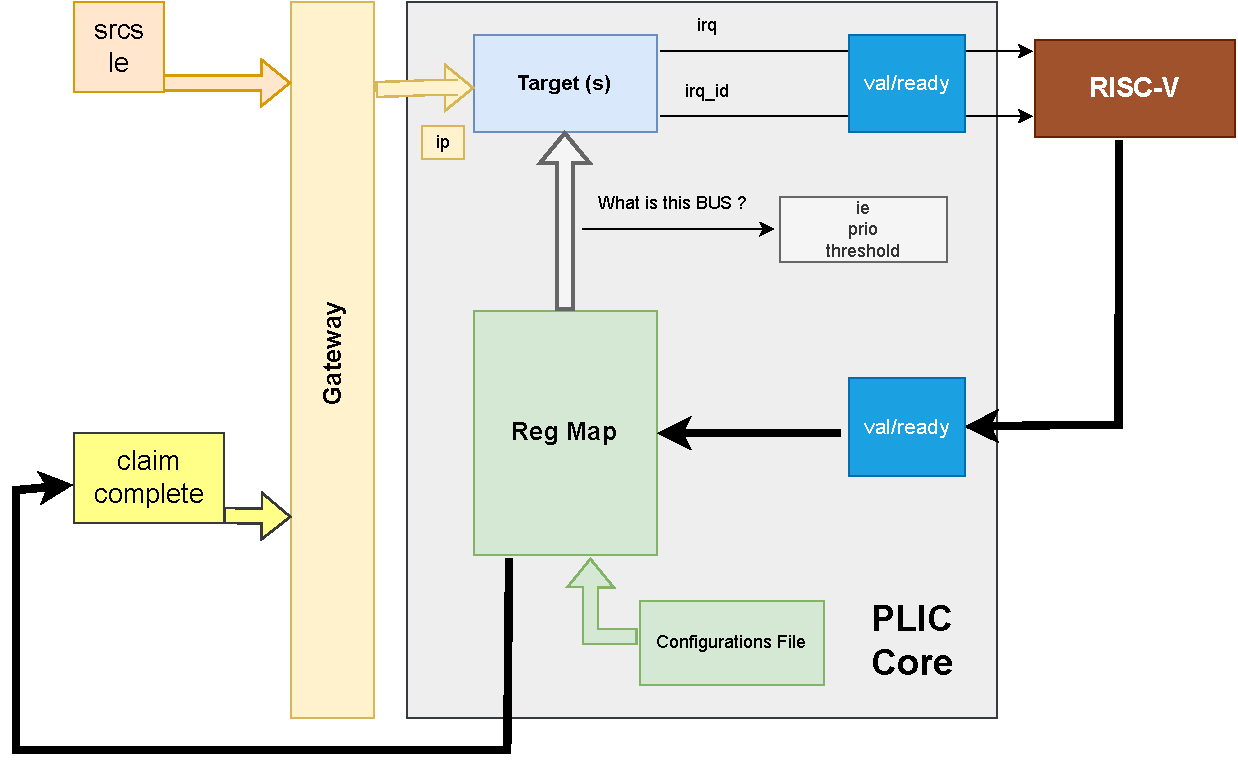
\includegraphics[width=0.95\textwidth]{./Figures/block_diagram.pdf}
  \caption{Block Diagram.}
  \label{fig:block_diagram}
\end{figure}


As we see in the figure \ref{fig:block_diagram}, there is also a block Reg Map (Register Map). It is used to store a particular interrupt is enabled or not, what is its priority, what is the threshold of the target to take that interrupt? etc. We program all this stuff using configuration file. At last, Processor also tells PLIC core that particular interrupt is taken and PLIC takes action to mark it as complete. 
